\chapter{Proposed Solution}

\begin{chapquote}{Jim Barksdale}
If we have data, let’s look at data. If all we have are opinions, let’s go with mine.
\end{chapquote}

\section{Introduction}

Perform a data-driven analysis required to develop a collection of tools
that are good enough to run in a lightning network node with daily activity. 
This section describes an open-source framework for the definition and 
the collection of lightning network metrics.

Therefore, in order to implement this framework an analysis of the state 
of the art was required (described in Section \ref{sec:problem_and_state_of_the_art})
to better understand what are the informations that are more difficult 
to get from a researcher's point of view.

From our preliminary study, we found that information on how a node performs 
on a daily basis are difficult to get, due to the following problems:
\begin{itemize}
    \item Requires a direct interaction with \emph{node operators};\footnote{node operators are people that own a 
        lightning node that point to help the network in routing payments.}
    \item Data collection of this kind can leak of private data, and node operators
        do not want be expose to this risk.
\end{itemize}

So, in order to work around these problems our proposal defines in a 
public manner what data will be collected, and how these are analyzed. This 
definition process is done through a lnmetrics Request for Comments (RFC) 
called \emph{lnmetrics RFC}. Then, after the data are defined, the collection 
of this data is done with a public server with public API with the possibility 
to self-hosting the server on hardware with at least a Raspberry PI 2 capability.

In addition, in order to incentivize node operators to provide and share the 
information with one of the public servers available we write the tool that 
collect the information on the lightning node with the possibility to run 
in an offline mode, and only if and when the node operators want the data 
are shared with one of the servers chosen (or more than one server).
One of the reasons that make the possibility to run in an offline mode a good
the incentive for node operators to be part of the research is that they 
are seeking a tool to analyze the node performance in order to increase the profit of
their node.

The Figure \ref{fig:lnmetrics_process} shows as the general process of propose 
a solution with our framework looks like.

\begin{figure}
    \begin{center}
      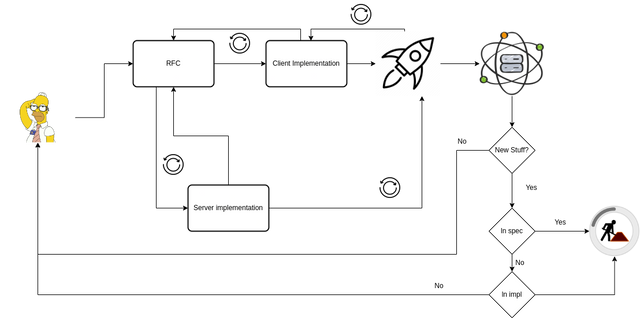
\includegraphics[scale=0.7]{imgs/lnmetrics-workflow-drawio.png}
    \end{center}
    \caption{Example of a process that uses lnmetrics.}
    \label{fig:lnmetrics_process}
\end{figure}

The suggested process to propose a new metrics described in the Figure \ref{fig:lnmetrics_process}
is composed by the following steps:

\begin{itemize}
    \item {\bf Data Definition}:
    \item {\bf Client Implementation}:
    \item {\bf Analysis Implementation}:
    \item {\bf Possible Proposal}:
\end{itemize}

\section{LNMetrics Request for Comments (RFC)}

The LNMetics Request for Comment (RFC) proposed is a more general idea of what 
it is already been done in the Lightning Network protocol definition. In fact,
this RFC is pointing to having the data description of what data are collected 
and how these data are used. It is not trying to define a 
standart of metrics for the lightning network, 
but more to incentivize discussion between people to achieve a better result.

\subsection{Data Definition}

Data definition is the most important part to propose a solution for a problem 
that required data analysis. Therefore, the data definition is a core 
part of the lnmetrics RFC process as the Figure \ref{fig:lnmetrics_process}
shows, and the process to propose a new \emph{metric} is composed from 
the following parts:

\begin{itemize}
    \item {\bf Metric Introduction}: An Introduction of the area that the metrics are targeting;
    \item {\bf Input Metric}: Data definition of the data that the researchers need. The data definition is done through a \emph{JSON schema}, and
    \item {\bf Output Metric}: Data definition of the data that the research point to return as a result. 
\end{itemize}

Ideally, the Metric proposal needs to be supported by a reference implementation to 
allow people to be part of the research by running the tool provided, and 
to support the RFC discussion.

However, at this time the problem on how to easily integrate new metrics inside the 
existing code is an open problem, and a possible solution is to allow the server 
to support a \emph{plugin protocol} that allow any person to extend the existing 
server with additional features.
In conclusion, when the new metric has been proposed inside the RFC a discussion between interested 
group of people need to be done in order to try to improve and verify the proposal, but if this is not possible
the proposal can be accepted directly by providing a reference implementation of the metrics proposed.

\section{Data Collection with LNMetrics Client}
\label{sec:lnmetrics_client}

A LNMetrics client is a generic concept of a tool that is able to collect one or more metrics 
defined inside the RFC, and allow a node operator or anyone that runs a lightning node
to collect data and share it with an analysis system described in Section \ref{sec:lnmetrics_server}.
In order to support our proposal a generic solution implemented in \emph{Go language} is provided 
and available on Github at \url{https://github.com/LNOpenMetrics/go-lnmetrics.reporter}, where we was able 
to provide a generic solution and allow the support of a generic metric concept 
by implementing the metric as interface defined as the Code \ref{code:lnmetric_client_inter} shows.

\begin{lstlisting}[language=go, basicstyle=\small,
                  caption={Metric interface provided in our client reference implementation.}, 
                  label={code:lnmetric_client_inter}]
// All the metrics need to respect this interface
type Metric interface {
    // return the unique name that the metrics has
    MetricName() *string
    // called when the metrics is initialized from 
    // the lightning node
    OnInit(lightning client.Client) error
    // called when the node is shutting down
    OnStop(msg *Msg, lightning client.Client) error
    // used to make the actual status of the metrics
    // persistent
    MakePersistent() error
    // called when the metrics is ready to be published
    UploadOnRepo(client *graphql.Client, 
        lightning client.Client) error
    // called when the metrics for the specific node 
    // need to be initialized on the server
    InitOnRepo(client *graphql.Client, 
        lightning client.Client) error
    // call that the lightning node use when it is 
    // time to update the metrics with new data
    Update(lightning client.Client) error
    // a more specific method to be able to call the 
    // update metrics with a specific message that allow 
    // to pass more information to the update method
    UpdateWithMsg(message *Msg, 
        lightning client.Client) error
    ToMap() (map[string]any, error)
    ToJSON() (string, error)
    // allow to perform data migration from an old 
    // data version to a new one
    Migrate(payload map[string]any) error
}
\end{lstlisting}

The LNMetrics client provided uses the core lightning plugin API
that allow us to easily integrate the client with the core lightning deamon 
and run the metrics client as part of the node itself. 
In addition, in order to allow an easy developmen of the plugin a 
Go API for core lightning is also provided, and available on 
Github at \url{https://github.com/vincenzopalazzo/cln4go}.

When the plugin is started a setup operation is performed, by creating a 
metrics database where the plugin make persistent the informations 
across node restarts, and also to support the offline mode feature. 
The database choosed is \emph{leveldb} that is a \emph{NO SQL} database 
that allow to store in an efficent way the data as key value and preserve
the disk space with a compression algorithm built-in the database itlsef.
In fact, our client implementation is havly based on the 
compression feature in order to preserve and allow anyone to 
run the tool. 

In the Figure (TODO add reference) it is shows how much space is 
consumed by the database in order to store 3 months of data on the server. 

TODO: put the figure here!

\section{LNMetrics Data Analsys}
\label{sec:lnmetrics_server}

After the data are collected by the LNMetrics client described in \ref{sec:lnmetrics_client}
our proposal is to aggregate the data in a server with public API where the data are 
public accessible to everyone. In this section there is a discussion of 
the server solution provided.

\section{Local Reputation Metric}

In this section is described our case study develop with the our metrics, and
in order to address a basic issue that we noted while we was running a lightning
node on the Bitcoin Network. 

\subsection{Problem}

When a new user want to run a lightning node from scratch at the moment it is 
difficult choose with what kind of peers if is a good incentivize to open a channel with. 

The choise of a good peer is important in this case because open a channel 
required to lock some bitcoin in a channel and also pay \emph{on-chain}\footnote{on chain fee are the fee that the Bitcoin network take in order to validate a block.} 
fe.

\subsection{Data Definition}

% FIXME: describe the data definition

\subsection{Reference Implementation}

% FIXME: Describe how the plugin works under the hood

\subsection{Data Analsys}

% FIXME: Describe a little bit how the data are analyzed
